\begin{blocksection}
\question Give the environment diagram and console output that result from running the following code.

\begin{lstlisting}
x = 20
def foo(y):
    x = 5
    if y == 5:
        return lambda y: x + y
    else:
        print('hello!')

y = foo(5)
x = y(7)
z = foo(7)
\end{lstlisting}

\begin{solution}[2in]
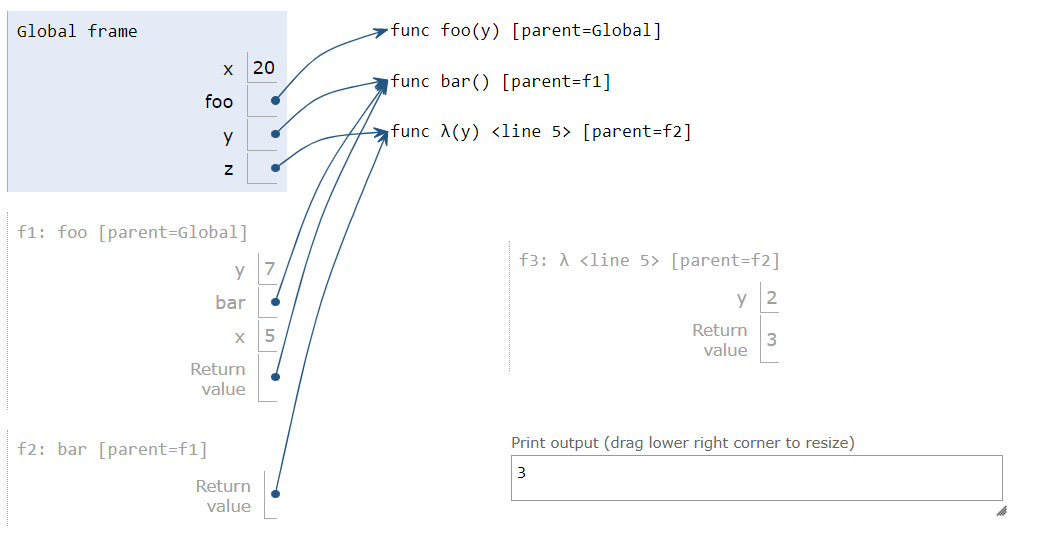
\includegraphics[scale=0.5]{foobar.png}
\\
\url{https://tinyurl.com/4dkbpnyc}
\end{solution}
\end{blocksection}